
% Default to the notebook output style

    


% Inherit from the specified cell style.




    
\documentclass[11pt]{article}

    
    
    \usepackage[T1]{fontenc}
    % Nicer default font (+ math font) than Computer Modern for most use cases
    \usepackage{mathpazo}

    % Basic figure setup, for now with no caption control since it's done
    % automatically by Pandoc (which extracts ![](path) syntax from Markdown).
    \usepackage{graphicx}
    % We will generate all images so they have a width \maxwidth. This means
    % that they will get their normal width if they fit onto the page, but
    % are scaled down if they would overflow the margins.
    \makeatletter
    \def\maxwidth{\ifdim\Gin@nat@width>\linewidth\linewidth
    \else\Gin@nat@width\fi}
    \makeatother
    \let\Oldincludegraphics\includegraphics
    % Set max figure width to be 80% of text width, for now hardcoded.
    \renewcommand{\includegraphics}[1]{\Oldincludegraphics[width=.8\maxwidth]{#1}}
    % Ensure that by default, figures have no caption (until we provide a
    % proper Figure object with a Caption API and a way to capture that
    % in the conversion process - todo).
    \usepackage{caption}
    \DeclareCaptionLabelFormat{nolabel}{}
    \captionsetup{labelformat=nolabel}

    \usepackage{adjustbox} % Used to constrain images to a maximum size 
    \usepackage{xcolor} % Allow colors to be defined
    \usepackage{enumerate} % Needed for markdown enumerations to work
    \usepackage{geometry} % Used to adjust the document margins
    \usepackage{amsmath} % Equations
    \usepackage{amssymb} % Equations
    \usepackage{textcomp} % defines textquotesingle
    % Hack from http://tex.stackexchange.com/a/47451/13684:
    \AtBeginDocument{%
        \def\PYZsq{\textquotesingle}% Upright quotes in Pygmentized code
    }
    \usepackage{upquote} % Upright quotes for verbatim code
    \usepackage{eurosym} % defines \euro
    \usepackage[mathletters]{ucs} % Extended unicode (utf-8) support
    \usepackage[utf8x]{inputenc} % Allow utf-8 characters in the tex document
    \usepackage{fancyvrb} % verbatim replacement that allows latex
    \usepackage{grffile} % extends the file name processing of package graphics 
                         % to support a larger range 
    % The hyperref package gives us a pdf with properly built
    % internal navigation ('pdf bookmarks' for the table of contents,
    % internal cross-reference links, web links for URLs, etc.)
    \usepackage{hyperref}
    \usepackage{longtable} % longtable support required by pandoc >1.10
    \usepackage{booktabs}  % table support for pandoc > 1.12.2
    \usepackage[inline]{enumitem} % IRkernel/repr support (it uses the enumerate* environment)
    \usepackage[normalem]{ulem} % ulem is needed to support strikethroughs (\sout)
                                % normalem makes italics be italics, not underlines
    

    
    
    % Colors for the hyperref package
    \definecolor{urlcolor}{rgb}{0,.145,.698}
    \definecolor{linkcolor}{rgb}{.71,0.21,0.01}
    \definecolor{citecolor}{rgb}{.12,.54,.11}

    % ANSI colors
    \definecolor{ansi-black}{HTML}{3E424D}
    \definecolor{ansi-black-intense}{HTML}{282C36}
    \definecolor{ansi-red}{HTML}{E75C58}
    \definecolor{ansi-red-intense}{HTML}{B22B31}
    \definecolor{ansi-green}{HTML}{00A250}
    \definecolor{ansi-green-intense}{HTML}{007427}
    \definecolor{ansi-yellow}{HTML}{DDB62B}
    \definecolor{ansi-yellow-intense}{HTML}{B27D12}
    \definecolor{ansi-blue}{HTML}{208FFB}
    \definecolor{ansi-blue-intense}{HTML}{0065CA}
    \definecolor{ansi-magenta}{HTML}{D160C4}
    \definecolor{ansi-magenta-intense}{HTML}{A03196}
    \definecolor{ansi-cyan}{HTML}{60C6C8}
    \definecolor{ansi-cyan-intense}{HTML}{258F8F}
    \definecolor{ansi-white}{HTML}{C5C1B4}
    \definecolor{ansi-white-intense}{HTML}{A1A6B2}

    % commands and environments needed by pandoc snippets
    % extracted from the output of `pandoc -s`
    \providecommand{\tightlist}{%
      \setlength{\itemsep}{0pt}\setlength{\parskip}{0pt}}
    \DefineVerbatimEnvironment{Highlighting}{Verbatim}{commandchars=\\\{\}}
    % Add ',fontsize=\small' for more characters per line
    \newenvironment{Shaded}{}{}
    \newcommand{\KeywordTok}[1]{\textcolor[rgb]{0.00,0.44,0.13}{\textbf{{#1}}}}
    \newcommand{\DataTypeTok}[1]{\textcolor[rgb]{0.56,0.13,0.00}{{#1}}}
    \newcommand{\DecValTok}[1]{\textcolor[rgb]{0.25,0.63,0.44}{{#1}}}
    \newcommand{\BaseNTok}[1]{\textcolor[rgb]{0.25,0.63,0.44}{{#1}}}
    \newcommand{\FloatTok}[1]{\textcolor[rgb]{0.25,0.63,0.44}{{#1}}}
    \newcommand{\CharTok}[1]{\textcolor[rgb]{0.25,0.44,0.63}{{#1}}}
    \newcommand{\StringTok}[1]{\textcolor[rgb]{0.25,0.44,0.63}{{#1}}}
    \newcommand{\CommentTok}[1]{\textcolor[rgb]{0.38,0.63,0.69}{\textit{{#1}}}}
    \newcommand{\OtherTok}[1]{\textcolor[rgb]{0.00,0.44,0.13}{{#1}}}
    \newcommand{\AlertTok}[1]{\textcolor[rgb]{1.00,0.00,0.00}{\textbf{{#1}}}}
    \newcommand{\FunctionTok}[1]{\textcolor[rgb]{0.02,0.16,0.49}{{#1}}}
    \newcommand{\RegionMarkerTok}[1]{{#1}}
    \newcommand{\ErrorTok}[1]{\textcolor[rgb]{1.00,0.00,0.00}{\textbf{{#1}}}}
    \newcommand{\NormalTok}[1]{{#1}}
    
    % Additional commands for more recent versions of Pandoc
    \newcommand{\ConstantTok}[1]{\textcolor[rgb]{0.53,0.00,0.00}{{#1}}}
    \newcommand{\SpecialCharTok}[1]{\textcolor[rgb]{0.25,0.44,0.63}{{#1}}}
    \newcommand{\VerbatimStringTok}[1]{\textcolor[rgb]{0.25,0.44,0.63}{{#1}}}
    \newcommand{\SpecialStringTok}[1]{\textcolor[rgb]{0.73,0.40,0.53}{{#1}}}
    \newcommand{\ImportTok}[1]{{#1}}
    \newcommand{\DocumentationTok}[1]{\textcolor[rgb]{0.73,0.13,0.13}{\textit{{#1}}}}
    \newcommand{\AnnotationTok}[1]{\textcolor[rgb]{0.38,0.63,0.69}{\textbf{\textit{{#1}}}}}
    \newcommand{\CommentVarTok}[1]{\textcolor[rgb]{0.38,0.63,0.69}{\textbf{\textit{{#1}}}}}
    \newcommand{\VariableTok}[1]{\textcolor[rgb]{0.10,0.09,0.49}{{#1}}}
    \newcommand{\ControlFlowTok}[1]{\textcolor[rgb]{0.00,0.44,0.13}{\textbf{{#1}}}}
    \newcommand{\OperatorTok}[1]{\textcolor[rgb]{0.40,0.40,0.40}{{#1}}}
    \newcommand{\BuiltInTok}[1]{{#1}}
    \newcommand{\ExtensionTok}[1]{{#1}}
    \newcommand{\PreprocessorTok}[1]{\textcolor[rgb]{0.74,0.48,0.00}{{#1}}}
    \newcommand{\AttributeTok}[1]{\textcolor[rgb]{0.49,0.56,0.16}{{#1}}}
    \newcommand{\InformationTok}[1]{\textcolor[rgb]{0.38,0.63,0.69}{\textbf{\textit{{#1}}}}}
    \newcommand{\WarningTok}[1]{\textcolor[rgb]{0.38,0.63,0.69}{\textbf{\textit{{#1}}}}}
    
    
    % Define a nice break command that doesn't care if a line doesn't already
    % exist.
    \def\br{\hspace*{\fill} \\* }
    % Math Jax compatability definitions
    \def\gt{>}
    \def\lt{<}
    % Document parameters
    \title{convnets}
    
    
    

    % Pygments definitions
    
\makeatletter
\def\PY@reset{\let\PY@it=\relax \let\PY@bf=\relax%
    \let\PY@ul=\relax \let\PY@tc=\relax%
    \let\PY@bc=\relax \let\PY@ff=\relax}
\def\PY@tok#1{\csname PY@tok@#1\endcsname}
\def\PY@toks#1+{\ifx\relax#1\empty\else%
    \PY@tok{#1}\expandafter\PY@toks\fi}
\def\PY@do#1{\PY@bc{\PY@tc{\PY@ul{%
    \PY@it{\PY@bf{\PY@ff{#1}}}}}}}
\def\PY#1#2{\PY@reset\PY@toks#1+\relax+\PY@do{#2}}

\expandafter\def\csname PY@tok@w\endcsname{\def\PY@tc##1{\textcolor[rgb]{0.73,0.73,0.73}{##1}}}
\expandafter\def\csname PY@tok@c\endcsname{\let\PY@it=\textit\def\PY@tc##1{\textcolor[rgb]{0.25,0.50,0.50}{##1}}}
\expandafter\def\csname PY@tok@cp\endcsname{\def\PY@tc##1{\textcolor[rgb]{0.74,0.48,0.00}{##1}}}
\expandafter\def\csname PY@tok@k\endcsname{\let\PY@bf=\textbf\def\PY@tc##1{\textcolor[rgb]{0.00,0.50,0.00}{##1}}}
\expandafter\def\csname PY@tok@kp\endcsname{\def\PY@tc##1{\textcolor[rgb]{0.00,0.50,0.00}{##1}}}
\expandafter\def\csname PY@tok@kt\endcsname{\def\PY@tc##1{\textcolor[rgb]{0.69,0.00,0.25}{##1}}}
\expandafter\def\csname PY@tok@o\endcsname{\def\PY@tc##1{\textcolor[rgb]{0.40,0.40,0.40}{##1}}}
\expandafter\def\csname PY@tok@ow\endcsname{\let\PY@bf=\textbf\def\PY@tc##1{\textcolor[rgb]{0.67,0.13,1.00}{##1}}}
\expandafter\def\csname PY@tok@nb\endcsname{\def\PY@tc##1{\textcolor[rgb]{0.00,0.50,0.00}{##1}}}
\expandafter\def\csname PY@tok@nf\endcsname{\def\PY@tc##1{\textcolor[rgb]{0.00,0.00,1.00}{##1}}}
\expandafter\def\csname PY@tok@nc\endcsname{\let\PY@bf=\textbf\def\PY@tc##1{\textcolor[rgb]{0.00,0.00,1.00}{##1}}}
\expandafter\def\csname PY@tok@nn\endcsname{\let\PY@bf=\textbf\def\PY@tc##1{\textcolor[rgb]{0.00,0.00,1.00}{##1}}}
\expandafter\def\csname PY@tok@ne\endcsname{\let\PY@bf=\textbf\def\PY@tc##1{\textcolor[rgb]{0.82,0.25,0.23}{##1}}}
\expandafter\def\csname PY@tok@nv\endcsname{\def\PY@tc##1{\textcolor[rgb]{0.10,0.09,0.49}{##1}}}
\expandafter\def\csname PY@tok@no\endcsname{\def\PY@tc##1{\textcolor[rgb]{0.53,0.00,0.00}{##1}}}
\expandafter\def\csname PY@tok@nl\endcsname{\def\PY@tc##1{\textcolor[rgb]{0.63,0.63,0.00}{##1}}}
\expandafter\def\csname PY@tok@ni\endcsname{\let\PY@bf=\textbf\def\PY@tc##1{\textcolor[rgb]{0.60,0.60,0.60}{##1}}}
\expandafter\def\csname PY@tok@na\endcsname{\def\PY@tc##1{\textcolor[rgb]{0.49,0.56,0.16}{##1}}}
\expandafter\def\csname PY@tok@nt\endcsname{\let\PY@bf=\textbf\def\PY@tc##1{\textcolor[rgb]{0.00,0.50,0.00}{##1}}}
\expandafter\def\csname PY@tok@nd\endcsname{\def\PY@tc##1{\textcolor[rgb]{0.67,0.13,1.00}{##1}}}
\expandafter\def\csname PY@tok@s\endcsname{\def\PY@tc##1{\textcolor[rgb]{0.73,0.13,0.13}{##1}}}
\expandafter\def\csname PY@tok@sd\endcsname{\let\PY@it=\textit\def\PY@tc##1{\textcolor[rgb]{0.73,0.13,0.13}{##1}}}
\expandafter\def\csname PY@tok@si\endcsname{\let\PY@bf=\textbf\def\PY@tc##1{\textcolor[rgb]{0.73,0.40,0.53}{##1}}}
\expandafter\def\csname PY@tok@se\endcsname{\let\PY@bf=\textbf\def\PY@tc##1{\textcolor[rgb]{0.73,0.40,0.13}{##1}}}
\expandafter\def\csname PY@tok@sr\endcsname{\def\PY@tc##1{\textcolor[rgb]{0.73,0.40,0.53}{##1}}}
\expandafter\def\csname PY@tok@ss\endcsname{\def\PY@tc##1{\textcolor[rgb]{0.10,0.09,0.49}{##1}}}
\expandafter\def\csname PY@tok@sx\endcsname{\def\PY@tc##1{\textcolor[rgb]{0.00,0.50,0.00}{##1}}}
\expandafter\def\csname PY@tok@m\endcsname{\def\PY@tc##1{\textcolor[rgb]{0.40,0.40,0.40}{##1}}}
\expandafter\def\csname PY@tok@gh\endcsname{\let\PY@bf=\textbf\def\PY@tc##1{\textcolor[rgb]{0.00,0.00,0.50}{##1}}}
\expandafter\def\csname PY@tok@gu\endcsname{\let\PY@bf=\textbf\def\PY@tc##1{\textcolor[rgb]{0.50,0.00,0.50}{##1}}}
\expandafter\def\csname PY@tok@gd\endcsname{\def\PY@tc##1{\textcolor[rgb]{0.63,0.00,0.00}{##1}}}
\expandafter\def\csname PY@tok@gi\endcsname{\def\PY@tc##1{\textcolor[rgb]{0.00,0.63,0.00}{##1}}}
\expandafter\def\csname PY@tok@gr\endcsname{\def\PY@tc##1{\textcolor[rgb]{1.00,0.00,0.00}{##1}}}
\expandafter\def\csname PY@tok@ge\endcsname{\let\PY@it=\textit}
\expandafter\def\csname PY@tok@gs\endcsname{\let\PY@bf=\textbf}
\expandafter\def\csname PY@tok@gp\endcsname{\let\PY@bf=\textbf\def\PY@tc##1{\textcolor[rgb]{0.00,0.00,0.50}{##1}}}
\expandafter\def\csname PY@tok@go\endcsname{\def\PY@tc##1{\textcolor[rgb]{0.53,0.53,0.53}{##1}}}
\expandafter\def\csname PY@tok@gt\endcsname{\def\PY@tc##1{\textcolor[rgb]{0.00,0.27,0.87}{##1}}}
\expandafter\def\csname PY@tok@err\endcsname{\def\PY@bc##1{\setlength{\fboxsep}{0pt}\fcolorbox[rgb]{1.00,0.00,0.00}{1,1,1}{\strut ##1}}}
\expandafter\def\csname PY@tok@kc\endcsname{\let\PY@bf=\textbf\def\PY@tc##1{\textcolor[rgb]{0.00,0.50,0.00}{##1}}}
\expandafter\def\csname PY@tok@kd\endcsname{\let\PY@bf=\textbf\def\PY@tc##1{\textcolor[rgb]{0.00,0.50,0.00}{##1}}}
\expandafter\def\csname PY@tok@kn\endcsname{\let\PY@bf=\textbf\def\PY@tc##1{\textcolor[rgb]{0.00,0.50,0.00}{##1}}}
\expandafter\def\csname PY@tok@kr\endcsname{\let\PY@bf=\textbf\def\PY@tc##1{\textcolor[rgb]{0.00,0.50,0.00}{##1}}}
\expandafter\def\csname PY@tok@bp\endcsname{\def\PY@tc##1{\textcolor[rgb]{0.00,0.50,0.00}{##1}}}
\expandafter\def\csname PY@tok@fm\endcsname{\def\PY@tc##1{\textcolor[rgb]{0.00,0.00,1.00}{##1}}}
\expandafter\def\csname PY@tok@vc\endcsname{\def\PY@tc##1{\textcolor[rgb]{0.10,0.09,0.49}{##1}}}
\expandafter\def\csname PY@tok@vg\endcsname{\def\PY@tc##1{\textcolor[rgb]{0.10,0.09,0.49}{##1}}}
\expandafter\def\csname PY@tok@vi\endcsname{\def\PY@tc##1{\textcolor[rgb]{0.10,0.09,0.49}{##1}}}
\expandafter\def\csname PY@tok@vm\endcsname{\def\PY@tc##1{\textcolor[rgb]{0.10,0.09,0.49}{##1}}}
\expandafter\def\csname PY@tok@sa\endcsname{\def\PY@tc##1{\textcolor[rgb]{0.73,0.13,0.13}{##1}}}
\expandafter\def\csname PY@tok@sb\endcsname{\def\PY@tc##1{\textcolor[rgb]{0.73,0.13,0.13}{##1}}}
\expandafter\def\csname PY@tok@sc\endcsname{\def\PY@tc##1{\textcolor[rgb]{0.73,0.13,0.13}{##1}}}
\expandafter\def\csname PY@tok@dl\endcsname{\def\PY@tc##1{\textcolor[rgb]{0.73,0.13,0.13}{##1}}}
\expandafter\def\csname PY@tok@s2\endcsname{\def\PY@tc##1{\textcolor[rgb]{0.73,0.13,0.13}{##1}}}
\expandafter\def\csname PY@tok@sh\endcsname{\def\PY@tc##1{\textcolor[rgb]{0.73,0.13,0.13}{##1}}}
\expandafter\def\csname PY@tok@s1\endcsname{\def\PY@tc##1{\textcolor[rgb]{0.73,0.13,0.13}{##1}}}
\expandafter\def\csname PY@tok@mb\endcsname{\def\PY@tc##1{\textcolor[rgb]{0.40,0.40,0.40}{##1}}}
\expandafter\def\csname PY@tok@mf\endcsname{\def\PY@tc##1{\textcolor[rgb]{0.40,0.40,0.40}{##1}}}
\expandafter\def\csname PY@tok@mh\endcsname{\def\PY@tc##1{\textcolor[rgb]{0.40,0.40,0.40}{##1}}}
\expandafter\def\csname PY@tok@mi\endcsname{\def\PY@tc##1{\textcolor[rgb]{0.40,0.40,0.40}{##1}}}
\expandafter\def\csname PY@tok@il\endcsname{\def\PY@tc##1{\textcolor[rgb]{0.40,0.40,0.40}{##1}}}
\expandafter\def\csname PY@tok@mo\endcsname{\def\PY@tc##1{\textcolor[rgb]{0.40,0.40,0.40}{##1}}}
\expandafter\def\csname PY@tok@ch\endcsname{\let\PY@it=\textit\def\PY@tc##1{\textcolor[rgb]{0.25,0.50,0.50}{##1}}}
\expandafter\def\csname PY@tok@cm\endcsname{\let\PY@it=\textit\def\PY@tc##1{\textcolor[rgb]{0.25,0.50,0.50}{##1}}}
\expandafter\def\csname PY@tok@cpf\endcsname{\let\PY@it=\textit\def\PY@tc##1{\textcolor[rgb]{0.25,0.50,0.50}{##1}}}
\expandafter\def\csname PY@tok@c1\endcsname{\let\PY@it=\textit\def\PY@tc##1{\textcolor[rgb]{0.25,0.50,0.50}{##1}}}
\expandafter\def\csname PY@tok@cs\endcsname{\let\PY@it=\textit\def\PY@tc##1{\textcolor[rgb]{0.25,0.50,0.50}{##1}}}

\def\PYZbs{\char`\\}
\def\PYZus{\char`\_}
\def\PYZob{\char`\{}
\def\PYZcb{\char`\}}
\def\PYZca{\char`\^}
\def\PYZam{\char`\&}
\def\PYZlt{\char`\<}
\def\PYZgt{\char`\>}
\def\PYZsh{\char`\#}
\def\PYZpc{\char`\%}
\def\PYZdl{\char`\$}
\def\PYZhy{\char`\-}
\def\PYZsq{\char`\'}
\def\PYZdq{\char`\"}
\def\PYZti{\char`\~}
% for compatibility with earlier versions
\def\PYZat{@}
\def\PYZlb{[}
\def\PYZrb{]}
\makeatother


    % Exact colors from NB
    \definecolor{incolor}{rgb}{0.0, 0.0, 0.5}
    \definecolor{outcolor}{rgb}{0.545, 0.0, 0.0}



    
    % Prevent overflowing lines due to hard-to-break entities
    \sloppy 
    % Setup hyperref package
    \hypersetup{
      breaklinks=true,  % so long urls are correctly broken across lines
      colorlinks=true,
      urlcolor=urlcolor,
      linkcolor=linkcolor,
      citecolor=citecolor,
      }
    % Slightly bigger margins than the latex defaults
    
    \geometry{verbose,tmargin=1in,bmargin=1in,lmargin=1in,rmargin=1in}
    
    

    \begin{document}
    
    
    \maketitle
    
    

    
    Plan: * 3-minute introduction to Neural Networks * A sequence of
operations * or in details DAG * Training: backpropagation * Convolution
layers: * Motivation: * FFT? * Filters? * Params: * Paddings * spartial
conv * Layers * formula * kernel dims * Convnets in CV: * MNIST *
Convnets in NLP: * character-level LM

    \hypertarget{sieci-konwolucyjne-w-przetwarzaniu-obrazuxf3w-i-tekstu}{%
\section{Sieci Konwolucyjne w przetwarzaniu obrazów i
tekstu}\label{sieci-konwolucyjne-w-przetwarzaniu-obrazuxf3w-i-tekstu}}

\hypertarget{tomasz-dwojak}{%
\subsubsection{Tomasz Dwojak}\label{tomasz-dwojak}}

\hypertarget{kwietnia-2018}{%
\subsubsection{24 kwietnia 2018}\label{kwietnia-2018}}

    \hypertarget{wprowadzenie-do-nns}{%
\subsubsection{Wprowadzenie do NNs}\label{wprowadzenie-do-nns}}

    \begin{itemize}
\tightlist
\item
  podstawowe klocki: warstawy
\item
  układanie puzzli z klocków
\item
  wejście: \(x \in {R}^{n \cdot m \cdot k \cdot l}\) -
  \href{https://stats.stackexchange.com/questions/198061/why-the-sudden-fascination-with-tensors}{tensor}:
\item
  0D tensor to skalar,
\item
  1D tensor to wektor,
\item
  2D tensor to macierz\ldots{}
\item
  4D tensor to \emph{macierz macierzy}
\end{itemize}

    \begin{Verbatim}[commandchars=\\\{\}]
{\color{incolor}In [{\color{incolor}26}]:} \PY{k+kn}{import} \PY{n+nn}{os}
         \PY{k+kn}{import} \PY{n+nn}{struct}
         \PY{k+kn}{import} \PY{n+nn}{numpy} \PY{k}{as} \PY{n+nn}{np}
         
         \PY{k}{def} \PY{n+nf}{readMnist}\PY{p}{(}\PY{n}{dataset} \PY{o}{=} \PY{l+s+s2}{\PYZdq{}}\PY{l+s+s2}{training}\PY{l+s+s2}{\PYZdq{}}\PY{p}{,} \PY{n}{path} \PY{o}{=} \PY{l+s+s2}{\PYZdq{}}\PY{l+s+s2}{.}\PY{l+s+s2}{\PYZdq{}}\PY{p}{)}\PY{p}{:}
             \PY{l+s+sd}{\PYZdq{}\PYZdq{}\PYZdq{}}
         \PY{l+s+sd}{    Python function for importing the MNIST data set.  It returns an iterator}
         \PY{l+s+sd}{    of 2\PYZhy{}tuples with the first element being the label and the second element}
         \PY{l+s+sd}{    being a numpy.uint8 2D array of pixel data for the given image.}
         \PY{l+s+sd}{    \PYZdq{}\PYZdq{}\PYZdq{}}
         
             \PY{k}{if} \PY{n}{dataset} \PY{o+ow}{is} \PY{l+s+s2}{\PYZdq{}}\PY{l+s+s2}{training}\PY{l+s+s2}{\PYZdq{}}\PY{p}{:}
                 \PY{n}{fname\PYZus{}img} \PY{o}{=} \PY{n}{os}\PY{o}{.}\PY{n}{path}\PY{o}{.}\PY{n}{join}\PY{p}{(}\PY{n}{path}\PY{p}{,} \PY{l+s+s1}{\PYZsq{}}\PY{l+s+s1}{train\PYZhy{}images\PYZhy{}idx3\PYZhy{}ubyte}\PY{l+s+s1}{\PYZsq{}}\PY{p}{)}
                 \PY{n}{fname\PYZus{}lbl} \PY{o}{=} \PY{n}{os}\PY{o}{.}\PY{n}{path}\PY{o}{.}\PY{n}{join}\PY{p}{(}\PY{n}{path}\PY{p}{,} \PY{l+s+s1}{\PYZsq{}}\PY{l+s+s1}{train\PYZhy{}labels\PYZhy{}idx1\PYZhy{}ubyte}\PY{l+s+s1}{\PYZsq{}}\PY{p}{)}
             \PY{k}{elif} \PY{n}{dataset} \PY{o+ow}{is} \PY{l+s+s2}{\PYZdq{}}\PY{l+s+s2}{testing}\PY{l+s+s2}{\PYZdq{}}\PY{p}{:}
                 \PY{n}{fname\PYZus{}img} \PY{o}{=} \PY{n}{os}\PY{o}{.}\PY{n}{path}\PY{o}{.}\PY{n}{join}\PY{p}{(}\PY{n}{path}\PY{p}{,} \PY{l+s+s1}{\PYZsq{}}\PY{l+s+s1}{t10k\PYZhy{}images\PYZhy{}idx3\PYZhy{}ubyte}\PY{l+s+s1}{\PYZsq{}}\PY{p}{)}
                 \PY{n}{fname\PYZus{}lbl} \PY{o}{=} \PY{n}{os}\PY{o}{.}\PY{n}{path}\PY{o}{.}\PY{n}{join}\PY{p}{(}\PY{n}{path}\PY{p}{,} \PY{l+s+s1}{\PYZsq{}}\PY{l+s+s1}{t10k\PYZhy{}labels\PYZhy{}idx1\PYZhy{}ubyte}\PY{l+s+s1}{\PYZsq{}}\PY{p}{)}
             \PY{k}{else}\PY{p}{:}
                 \PY{k}{raise} \PY{n+ne}{ValueError}\PY{p}{(}\PY{l+s+s2}{\PYZdq{}}\PY{l+s+s2}{dataset must be }\PY{l+s+s2}{\PYZsq{}}\PY{l+s+s2}{testing}\PY{l+s+s2}{\PYZsq{}}\PY{l+s+s2}{ or }\PY{l+s+s2}{\PYZsq{}}\PY{l+s+s2}{training}\PY{l+s+s2}{\PYZsq{}}\PY{l+s+s2}{\PYZdq{}}\PY{p}{)}
         
             \PY{c+c1}{\PYZsh{} Load everything in some numpy arrays}
             \PY{k}{with} \PY{n+nb}{open}\PY{p}{(}\PY{n}{fname\PYZus{}lbl}\PY{p}{,} \PY{l+s+s1}{\PYZsq{}}\PY{l+s+s1}{rb}\PY{l+s+s1}{\PYZsq{}}\PY{p}{)} \PY{k}{as} \PY{n}{flbl}\PY{p}{:}
                 \PY{n}{magic}\PY{p}{,} \PY{n}{num} \PY{o}{=} \PY{n}{struct}\PY{o}{.}\PY{n}{unpack}\PY{p}{(}\PY{l+s+s2}{\PYZdq{}}\PY{l+s+s2}{\PYZgt{}II}\PY{l+s+s2}{\PYZdq{}}\PY{p}{,} \PY{n}{flbl}\PY{o}{.}\PY{n}{read}\PY{p}{(}\PY{l+m+mi}{8}\PY{p}{)}\PY{p}{)}
                 \PY{n}{lbl} \PY{o}{=} \PY{n}{np}\PY{o}{.}\PY{n}{fromfile}\PY{p}{(}\PY{n}{flbl}\PY{p}{,} \PY{n}{dtype}\PY{o}{=}\PY{n}{np}\PY{o}{.}\PY{n}{int8}\PY{p}{)}
         
             \PY{k}{with} \PY{n+nb}{open}\PY{p}{(}\PY{n}{fname\PYZus{}img}\PY{p}{,} \PY{l+s+s1}{\PYZsq{}}\PY{l+s+s1}{rb}\PY{l+s+s1}{\PYZsq{}}\PY{p}{)} \PY{k}{as} \PY{n}{fimg}\PY{p}{:}
                 \PY{n}{magic}\PY{p}{,} \PY{n}{num}\PY{p}{,} \PY{n}{rows}\PY{p}{,} \PY{n}{cols} \PY{o}{=} \PY{n}{struct}\PY{o}{.}\PY{n}{unpack}\PY{p}{(}\PY{l+s+s2}{\PYZdq{}}\PY{l+s+s2}{\PYZgt{}IIII}\PY{l+s+s2}{\PYZdq{}}\PY{p}{,} \PY{n}{fimg}\PY{o}{.}\PY{n}{read}\PY{p}{(}\PY{l+m+mi}{16}\PY{p}{)}\PY{p}{)}
                 \PY{n}{img} \PY{o}{=} \PY{n}{np}\PY{o}{.}\PY{n}{fromfile}\PY{p}{(}\PY{n}{fimg}\PY{p}{,} \PY{n}{dtype}\PY{o}{=}\PY{n}{np}\PY{o}{.}\PY{n}{uint8}\PY{p}{)}\PY{o}{.}\PY{n}{reshape}\PY{p}{(}\PY{n+nb}{len}\PY{p}{(}\PY{n}{lbl}\PY{p}{)}\PY{p}{,} \PY{n}{rows}\PY{p}{,} \PY{n}{cols}\PY{p}{)}
                 \PY{n}{img} \PY{o}{=} \PY{n}{img}\PY{o}{.}\PY{n}{astype}\PY{p}{(}\PY{n}{np}\PY{o}{.}\PY{n}{float32}\PY{p}{)}
         
             \PY{n}{get\PYZus{}img} \PY{o}{=} \PY{k}{lambda} \PY{n}{idx}\PY{p}{:} \PY{p}{(}\PY{n}{lbl}\PY{p}{[}\PY{n}{idx}\PY{p}{]}\PY{p}{,} \PY{n}{img}\PY{p}{[}\PY{n}{idx}\PY{p}{]}\PY{p}{)}
         
             \PY{k}{return} \PY{p}{[}\PY{n}{get\PYZus{}img}\PY{p}{(}\PY{n}{i}\PY{p}{)} \PY{k}{for} \PY{n}{i} \PY{o+ow}{in} \PY{n+nb}{range}\PY{p}{(}\PY{n+nb}{len}\PY{p}{(}\PY{n}{lbl}\PY{p}{)}\PY{p}{)}\PY{p}{]}
\end{Verbatim}


    \begin{Verbatim}[commandchars=\\\{\}]
{\color{incolor}In [{\color{incolor}27}]:} \PY{k}{def} \PY{n+nf}{showImage}\PY{p}{(}\PY{n}{image}\PY{p}{)}\PY{p}{:}
             \PY{l+s+sd}{\PYZdq{}\PYZdq{}\PYZdq{}}
         \PY{l+s+sd}{    Render a given numpy.uint8 2D array of pixel data.}
         \PY{l+s+sd}{    \PYZdq{}\PYZdq{}\PYZdq{}}
             \PY{k+kn}{from} \PY{n+nn}{matplotlib} \PY{k}{import} \PY{n}{pyplot}
             \PY{k+kn}{import} \PY{n+nn}{matplotlib} \PY{k}{as} \PY{n+nn}{mpl}
             \PY{n}{fig} \PY{o}{=} \PY{n}{pyplot}\PY{o}{.}\PY{n}{figure}\PY{p}{(}\PY{p}{)}
             \PY{n}{ax} \PY{o}{=} \PY{n}{fig}\PY{o}{.}\PY{n}{add\PYZus{}subplot}\PY{p}{(}\PY{l+m+mi}{1}\PY{p}{,}\PY{l+m+mi}{1}\PY{p}{,}\PY{l+m+mi}{1}\PY{p}{)}
             \PY{n}{imgplot} \PY{o}{=} \PY{n}{ax}\PY{o}{.}\PY{n}{imshow}\PY{p}{(}\PY{n}{image}\PY{p}{,} \PY{n}{cmap}\PY{o}{=}\PY{n}{mpl}\PY{o}{.}\PY{n}{cm}\PY{o}{.}\PY{n}{Greys}\PY{p}{)}
             \PY{n}{imgplot}\PY{o}{.}\PY{n}{set\PYZus{}interpolation}\PY{p}{(}\PY{l+s+s1}{\PYZsq{}}\PY{l+s+s1}{nearest}\PY{l+s+s1}{\PYZsq{}}\PY{p}{)}
             \PY{n}{ax}\PY{o}{.}\PY{n}{xaxis}\PY{o}{.}\PY{n}{set\PYZus{}ticks\PYZus{}position}\PY{p}{(}\PY{l+s+s1}{\PYZsq{}}\PY{l+s+s1}{top}\PY{l+s+s1}{\PYZsq{}}\PY{p}{)}
             \PY{n}{ax}\PY{o}{.}\PY{n}{yaxis}\PY{o}{.}\PY{n}{set\PYZus{}ticks\PYZus{}position}\PY{p}{(}\PY{l+s+s1}{\PYZsq{}}\PY{l+s+s1}{left}\PY{l+s+s1}{\PYZsq{}}\PY{p}{)}
             \PY{n}{pyplot}\PY{o}{.}\PY{n}{show}\PY{p}{(}\PY{p}{)}
\end{Verbatim}


    \begin{Verbatim}[commandchars=\\\{\}]
{\color{incolor}In [{\color{incolor}30}]:} \PY{n}{training} \PY{o}{=} \PY{n}{readMnist}\PY{p}{(}\PY{p}{)}
         \PY{n+nb}{print}\PY{p}{(}\PY{n}{training}\PY{p}{[}\PY{l+m+mi}{0}\PY{p}{]}\PY{p}{[}\PY{l+m+mi}{1}\PY{p}{]}\PY{o}{.}\PY{n}{shape}\PY{p}{)}
\end{Verbatim}


    \begin{Verbatim}[commandchars=\\\{\}]
(28, 28)

    \end{Verbatim}

    Warstwy (ang. \emph{layers}): * liniowa: \$ x \leftarrow xW + b\$ *
element-wise: \$ x\cdot W\$ * nieliniowe (f. aktywacji): np.
\(x \leftarrow \tanh(x)\), \(x \leftarrow \sigma(x)\),
\(\DeclareMathOperator{\relu}{ReLU} x \leftarrow \relu(x)\) * pooling:,
np. max-pooling, ave-pooling * RNN: LSTM, GRU * Konwolucyjna: \(x * W\)

    \hypertarget{training}{%
\subsubsection{Training}\label{training}}

\begin{itemize}
\tightlist
\item
  forward
\item
  computing loss function, e.g.~MSE, CE
\item
  backward (back propagation)
\item
  update weights
\item
  repeat til some condition\ldots{}
\end{itemize}

    \begin{Verbatim}[commandchars=\\\{\}]
{\color{incolor}In [{\color{incolor}32}]:} \PY{k}{def} \PY{n+nf}{train\PYZus{}epoch}\PY{p}{(}\PY{n}{model}\PY{p}{,} \PY{n}{criterion}\PY{p}{,} \PY{n}{optimizer}\PY{p}{)}\PY{p}{:}
             \PY{n}{model}\PY{o}{.}\PY{n}{train}\PY{p}{(}\PY{p}{)}
             \PY{k}{for} \PY{n}{batch} \PY{o+ow}{in} \PY{n}{batch\PYZus{}generator}\PY{p}{(}\PY{p}{)}\PY{p}{:}
                 \PY{n}{optimizer}\PY{o}{.}\PY{n}{zero\PYZus{}grad}\PY{p}{(}\PY{p}{)}
                 
                 \PY{n}{inputs} \PY{o}{=} \PY{n}{Variable}\PY{p}{(}\PY{n}{torch}\PY{o}{.}\PY{n}{from\PYZus{}numpy}\PY{p}{(}\PY{n}{batch}\PY{p}{[}\PY{l+m+mi}{0}\PY{p}{]}\PY{p}{)}\PY{p}{)}
                 \PY{n}{labels} \PY{o}{=} \PY{n}{Variable}\PY{p}{(}\PY{n}{torch}\PY{o}{.}\PY{n}{from\PYZus{}numpy}\PY{p}{(}\PY{n}{batch}\PY{p}{[}\PY{l+m+mi}{1}\PY{p}{]}\PY{p}{)}\PY{p}{)}
                 
                 \PY{n}{outputs} \PY{o}{=} \PY{n}{model}\PY{p}{(}\PY{n}{inputs}\PY{p}{)}
                 \PY{n}{loss} \PY{o}{=} \PY{n}{criterion}\PY{p}{(}\PY{n}{outputs}\PY{p}{,} \PY{n}{labels}\PY{p}{)}
                 \PY{n}{loss}\PY{o}{.}\PY{n}{backward}\PY{p}{(}\PY{p}{)}
         
                 \PY{n}{optimizer}\PY{o}{.}\PY{n}{step}\PY{p}{(}\PY{p}{)}
\end{Verbatim}


    \hypertarget{images-in-ml}{%
\subsubsection{Images in ML}\label{images-in-ml}}

    \begin{Verbatim}[commandchars=\\\{\}]
{\color{incolor}In [{\color{incolor}20}]:} \PY{n}{showImage}\PY{p}{(}\PY{n}{training}\PY{p}{[}\PY{l+m+mi}{0}\PY{p}{]}\PY{p}{[}\PY{l+m+mi}{1}\PY{p}{]}\PY{p}{)}
\end{Verbatim}


    \begin{center}
    \adjustimage{max size={0.9\linewidth}{0.9\paperheight}}{output_11_0.png}
    \end{center}
    { \hspace*{\fill} \\}
    
    \begin{Verbatim}[commandchars=\\\{\}]
{\color{incolor}In [{\color{incolor}31}]:} \PY{n}{example} \PY{o}{=} \PY{l+s+s1}{\PYZsq{}}\PY{l+s+s1}{\PYZsq{}}
         \PY{n+nb}{print}\PY{p}{(}\PY{l+s+s1}{\PYZsq{}}\PY{l+s+se}{\PYZbs{}n}\PY{l+s+s1}{\PYZsq{}}\PY{o}{.}\PY{n}{join}\PY{p}{(}\PY{p}{[}\PY{l+s+s1}{\PYZsq{}}\PY{l+s+s1}{\PYZsq{}}\PY{o}{.}\PY{n}{join}\PY{p}{(}\PY{p}{[}\PY{n+nb}{str}\PY{p}{(}\PY{n+nb}{int}\PY{p}{(}\PY{n+nb}{bool}\PY{p}{(}\PY{n}{col}\PY{p}{)}\PY{p}{)}\PY{p}{)} \PY{k}{for} \PY{n}{col} \PY{o+ow}{in} \PY{n}{row}\PY{p}{]}\PY{p}{)} \PY{k}{for} \PY{n}{row} \PY{o+ow}{in} \PY{n}{training}\PY{p}{[}\PY{l+m+mi}{0}\PY{p}{]}\PY{p}{[}\PY{l+m+mi}{1}\PY{p}{]}\PY{p}{]}\PY{p}{)}\PY{p}{)}
\end{Verbatim}


    \begin{Verbatim}[commandchars=\\\{\}]
0000000000000000000000000000
0000000000000000000000000000
0000000000000000000000000000
0000000000000000000000000000
0000000000000000000000000000
0000000000001111111111110000
0000000011111111111111110000
0000000111111111111111100000
0000000111111111110000000000
0000000011111110110000000000
0000000001111100000000000000
0000000000011110000000000000
0000000000011110000000000000
0000000000001111110000000000
0000000000000111111000000000
0000000000000011111100000000
0000000000000001111100000000
0000000000000000011110000000
0000000000000011111110000000
0000000000001111111100000000
0000000000111111111000000000
0000000011111111110000000000
0000001111111111000000000000
0000111111111100000000000000
0000111111110000000000000000
0000000000000000000000000000
0000000000000000000000000000
0000000000000000000000000000

    \end{Verbatim}

    \hypertarget{convolutions}{%
\subsubsection{Convolutions}\label{convolutions}}

\[
s(t) = \int_{-\infty}^{+\infty}{x(a)w(t-a)da}
\]

\[
s(t) = (x * w)(t)
\]

    \[
s(t) = \sum_{a=-\infty}^{\infty}{x(a)w(t-a)}
\]

    \[
S(i, j) = (I * K)(i,j) = \sum_{m}\sum_{n}{I(m,n) \cdot K(i-m,j-n)}
\]

\[
S(i, j) = (K * I)(i,j) = \sum_{m}\sum_{n}{I(i-m, j-n) \cdot K(m,n)}
\]

\[
S(i, j) = (K * I)(i,j) = \sum_{m}\sum_{n}{I(i+m, j+n) \cdot K(m,n)}
\]

    \[
S(i, j) = (K * I)(i,j) = b + \sum_{m}{\sum_{n}{I(i+m, j+n) \cdot K(m,n)}}
\]

    \hypertarget{convnets}{%
\subsubsection{Convnets}\label{convnets}}

Previously, we had to find filters (a.k.a. kernels) manually:

    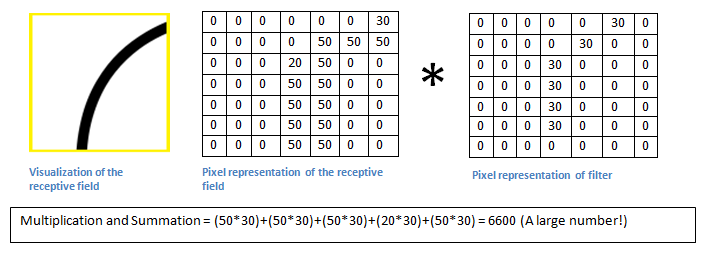
\includegraphics{FirstPixelMulitiplication.png}

    \includegraphics{./Convolution_schematic.gif}

    \begin{Verbatim}[commandchars=\\\{\}]
{\color{incolor}In [{\color{incolor}63}]:} \PY{n}{kernel} \PY{o}{=} \PY{p}{[}\PY{l+m+mf}{0.0}\PY{p}{,} \PY{l+m+mf}{1.0}\PY{p}{,} \PY{l+m+mf}{0.0}\PY{p}{,}
                   \PY{l+m+mf}{1.0}\PY{p}{,} \PY{l+m+mf}{0.0}\PY{p}{,} \PY{l+m+mf}{1.0}\PY{p}{,}
                   \PY{l+m+mf}{0.0}\PY{p}{,} \PY{l+m+mf}{1.0}\PY{p}{,} \PY{l+m+mf}{0.0}\PY{p}{]}
\end{Verbatim}


    \begin{Verbatim}[commandchars=\\\{\}]
{\color{incolor}In [{\color{incolor}64}]:} \PY{n}{inputs} \PY{o}{=} \PY{n}{Variable}\PY{p}{(}\PY{n}{torch}\PY{o}{.}\PY{n}{from\PYZus{}numpy}\PY{p}{(}\PY{n}{training}\PY{p}{[}\PY{l+m+mi}{0}\PY{p}{]}\PY{p}{[}\PY{l+m+mi}{1}\PY{p}{]}\PY{p}{)}\PY{p}{)}\PY{o}{.}\PY{n}{unsqueeze}\PY{p}{(}\PY{l+m+mi}{0}\PY{p}{)}\PY{o}{.}\PY{n}{unsqueeze}\PY{p}{(}\PY{l+m+mi}{0}\PY{p}{)}
         \PY{n}{vertical} \PY{o}{=} \PY{n}{nn}\PY{o}{.}\PY{n}{Conv2d}\PY{p}{(}\PY{l+m+mi}{1}\PY{p}{,} \PY{l+m+mi}{1}\PY{p}{,} \PY{l+m+mi}{3}\PY{p}{,} \PY{n}{padding}\PY{o}{=}\PY{l+m+mi}{1}\PY{p}{,} \PY{n}{bias}\PY{o}{=}\PY{k+kc}{False}\PY{p}{)}
         \PY{n}{vertical}\PY{o}{.}\PY{n}{weight}\PY{o}{.}\PY{n}{data} \PY{o}{=} \PY{n}{torch}\PY{o}{.}\PY{n}{from\PYZus{}numpy}\PY{p}{(}\PY{n}{np}\PY{o}{.}\PY{n}{array}\PY{p}{(}\PY{n}{kernel}\PY{p}{,} \PY{n}{dtype}\PY{o}{=}\PY{n}{np}\PY{o}{.}\PY{n}{float32}\PY{p}{)}\PY{o}{.}\PY{n}{reshape}\PY{p}{(}\PY{p}{(}\PY{l+m+mi}{1}\PY{p}{,} \PY{l+m+mi}{1}\PY{p}{,} \PY{l+m+mi}{3}\PY{p}{,} \PY{l+m+mi}{3}\PY{p}{)}\PY{p}{)}\PY{p}{)}
         \PY{n}{output} \PY{o}{=} \PY{n}{vertical}\PY{p}{(}\PY{n}{inputs}\PY{p}{)}
         \PY{n}{showImage}\PY{p}{(}\PY{n}{output}\PY{o}{.}\PY{n}{data}\PY{o}{.}\PY{n}{numpy}\PY{p}{(}\PY{p}{)}\PY{o}{.}\PY{n}{reshape}\PY{p}{(}\PY{p}{(}\PY{l+m+mi}{28}\PY{p}{,} \PY{l+m+mi}{28}\PY{p}{)}\PY{p}{)} \PY{o}{/} \PY{l+m+mi}{3}\PY{p}{)}
\end{Verbatim}


    \begin{center}
    \adjustimage{max size={0.9\linewidth}{0.9\paperheight}}{output_21_0.png}
    \end{center}
    { \hspace*{\fill} \\}
    
    \hypertarget{convnets-and-dl}{%
\subsubsection{Convnets and DL}\label{convnets-and-dl}}

let NN to learn its own filters!

    \[
Convnet \rightarrow activation \rightarrow pooling
\]

    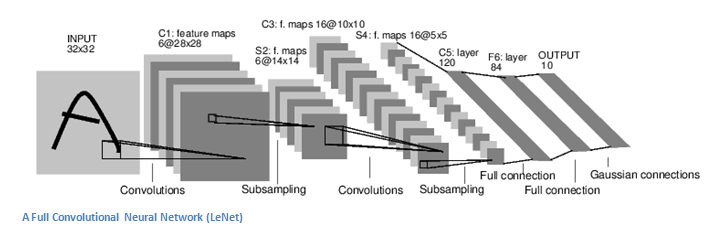
\includegraphics{./LeNet.png}

    \begin{Verbatim}[commandchars=\\\{\}]
{\color{incolor}In [{\color{incolor}67}]:} \PY{k}{class} \PY{n+nc}{LeNet}\PY{p}{(}\PY{n}{nn}\PY{o}{.}\PY{n}{Module}\PY{p}{)}\PY{p}{:}
             \PY{k}{def} \PY{n+nf}{\PYZus{}\PYZus{}init\PYZus{}\PYZus{}}\PY{p}{(}\PY{n+nb+bp}{self}\PY{p}{)}\PY{p}{:}
                 \PY{n+nb}{super}\PY{p}{(}\PY{n}{LeNet}\PY{p}{,} \PY{n+nb+bp}{self}\PY{p}{)}\PY{o}{.}\PY{n+nf+fm}{\PYZus{}\PYZus{}init\PYZus{}\PYZus{}}\PY{p}{(}\PY{p}{)}
                 \PY{n+nb+bp}{self}\PY{o}{.}\PY{n}{conv1} \PY{o}{=} \PY{n}{nn}\PY{o}{.}\PY{n}{Conv2d}\PY{p}{(}\PY{l+m+mi}{1}\PY{p}{,} \PY{l+m+mi}{6}\PY{p}{,} \PY{p}{(}\PY{l+m+mi}{5}\PY{p}{,}\PY{l+m+mi}{5}\PY{p}{)}\PY{p}{,} \PY{n}{padding}\PY{o}{=}\PY{l+m+mi}{2}\PY{p}{)}
                 \PY{n+nb+bp}{self}\PY{o}{.}\PY{n}{conv2} \PY{o}{=} \PY{n}{nn}\PY{o}{.}\PY{n}{Conv2d}\PY{p}{(}\PY{l+m+mi}{6}\PY{p}{,} \PY{l+m+mi}{16}\PY{p}{,} \PY{p}{(}\PY{l+m+mi}{5}\PY{p}{,}\PY{l+m+mi}{5}\PY{p}{)}\PY{p}{)}
                 \PY{n+nb+bp}{self}\PY{o}{.}\PY{n}{fc1}   \PY{o}{=} \PY{n}{nn}\PY{o}{.}\PY{n}{Linear}\PY{p}{(}\PY{l+m+mi}{16}\PY{o}{*}\PY{l+m+mi}{5}\PY{o}{*}\PY{l+m+mi}{5}\PY{p}{,} \PY{l+m+mi}{120}\PY{p}{)}
                 \PY{n+nb+bp}{self}\PY{o}{.}\PY{n}{fc2}   \PY{o}{=} \PY{n}{nn}\PY{o}{.}\PY{n}{Linear}\PY{p}{(}\PY{l+m+mi}{120}\PY{p}{,} \PY{l+m+mi}{84}\PY{p}{)}
                 \PY{n+nb+bp}{self}\PY{o}{.}\PY{n}{fc3}   \PY{o}{=} \PY{n}{nn}\PY{o}{.}\PY{n}{Linear}\PY{p}{(}\PY{l+m+mi}{84}\PY{p}{,} \PY{l+m+mi}{10}\PY{p}{)}
                 
             \PY{k}{def} \PY{n+nf}{forward}\PY{p}{(}\PY{n+nb+bp}{self}\PY{p}{,} \PY{n}{x}\PY{p}{)}\PY{p}{:}
                 \PY{n}{x} \PY{o}{=} \PY{n}{F}\PY{o}{.}\PY{n}{max\PYZus{}pool2d}\PY{p}{(}\PY{n}{F}\PY{o}{.}\PY{n}{relu}\PY{p}{(}\PY{n+nb+bp}{self}\PY{o}{.}\PY{n}{conv1}\PY{p}{(}\PY{n}{x}\PY{p}{)}\PY{p}{)}\PY{p}{,} \PY{p}{(}\PY{l+m+mi}{2}\PY{p}{,}\PY{l+m+mi}{2}\PY{p}{)}\PY{p}{)}
                 \PY{n}{x} \PY{o}{=} \PY{n}{F}\PY{o}{.}\PY{n}{max\PYZus{}pool2d}\PY{p}{(}\PY{n}{F}\PY{o}{.}\PY{n}{relu}\PY{p}{(}\PY{n+nb+bp}{self}\PY{o}{.}\PY{n}{conv2}\PY{p}{(}\PY{n}{x}\PY{p}{)}\PY{p}{)}\PY{p}{,} \PY{p}{(}\PY{l+m+mi}{2}\PY{p}{,}\PY{l+m+mi}{2}\PY{p}{)}\PY{p}{)}
                 \PY{n}{x} \PY{o}{=} \PY{n}{x}\PY{o}{.}\PY{n}{view}\PY{p}{(}\PY{o}{\PYZhy{}}\PY{l+m+mi}{1}\PY{p}{,} \PY{n+nb+bp}{self}\PY{o}{.}\PY{n}{num\PYZus{}flat\PYZus{}features}\PY{p}{(}\PY{n}{x}\PY{p}{)}\PY{p}{)}
                 \PY{n}{x} \PY{o}{=} \PY{n}{F}\PY{o}{.}\PY{n}{relu}\PY{p}{(}\PY{n+nb+bp}{self}\PY{o}{.}\PY{n}{fc1}\PY{p}{(}\PY{n}{x}\PY{p}{)}\PY{p}{)}
                 \PY{n}{x} \PY{o}{=} \PY{n}{F}\PY{o}{.}\PY{n}{relu}\PY{p}{(}\PY{n+nb+bp}{self}\PY{o}{.}\PY{n}{fc2}\PY{p}{(}\PY{n}{x}\PY{p}{)}\PY{p}{)}
                 \PY{n}{x} \PY{o}{=} \PY{n+nb+bp}{self}\PY{o}{.}\PY{n}{fc3}\PY{p}{(}\PY{n}{x}\PY{p}{)}
                 \PY{k}{return} \PY{n}{x}
\end{Verbatim}


    \hypertarget{alexnet}{%
\subsubsection{AlexNet}\label{alexnet}}

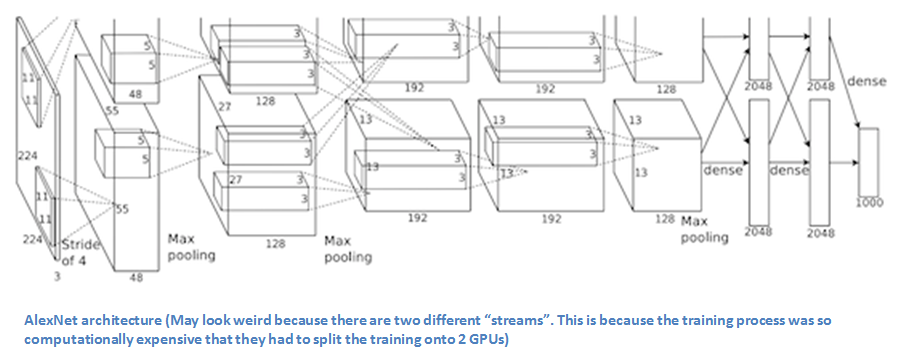
\includegraphics{./AlexNet.png}

    \begin{itemize}
\tightlist
\item
  Trained the network on ImageNet data, which contained over 15 million
  annotated images from a total of over 22,000 categories.
\item
  Used ReLU for the nonlinearity functions (Found to decrease training
  time as ReLUs are several times faster than the conventional tanh
  function).
\item
  Used data augmentation techniques that consisted of image
  translations, horizontal reflections, and patch extractions.
\item
  Implemented dropout layers in order to combat the problem of
  overfitting to the training data.
\item
  Trained the model using batch stochastic gradient descent, with
  specific values for momentum and weight decay.
\item
  Trained on two GTX 580 GPUs for five to six days.
\end{itemize}

    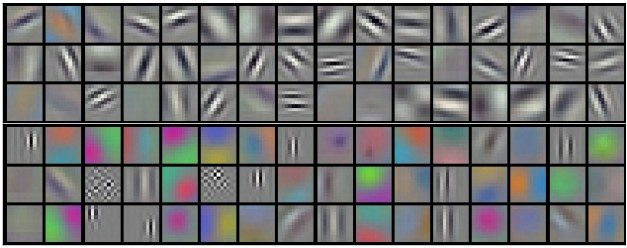
\includegraphics{./weights.jpeg}

    \hypertarget{googlenet}{%
\subsubsection{GoogLeNet}\label{googlenet}}

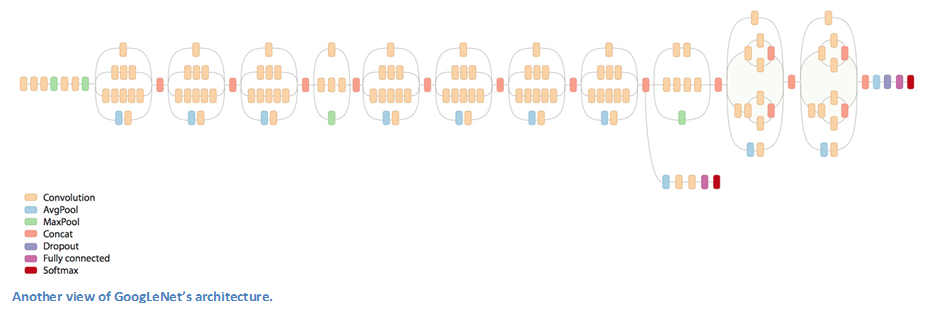
\includegraphics{./GoogLeNet.png}

    \hypertarget{inception}{%
\subsection{Inception}\label{inception}}

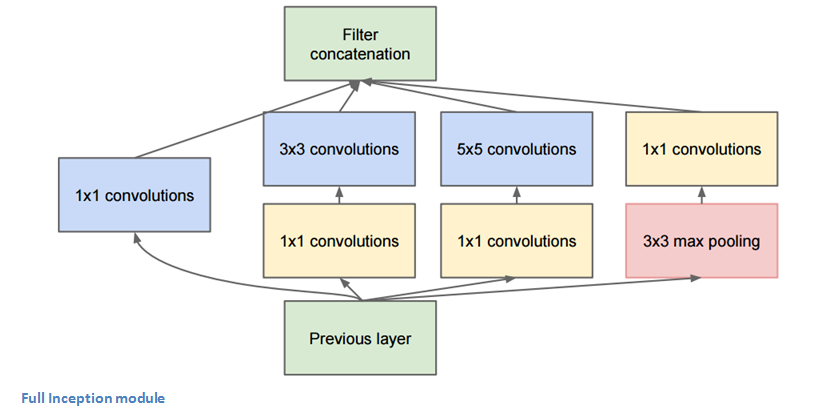
\includegraphics{./GoogLeNet3.png}

    \hypertarget{and-deeper}{%
\subsubsection{And deeper}\label{and-deeper}}

\begin{itemize}
\tightlist
\item
  ResNet (157 layers)
\item
  GANs
\item
  and many more\ldots{}
\end{itemize}

    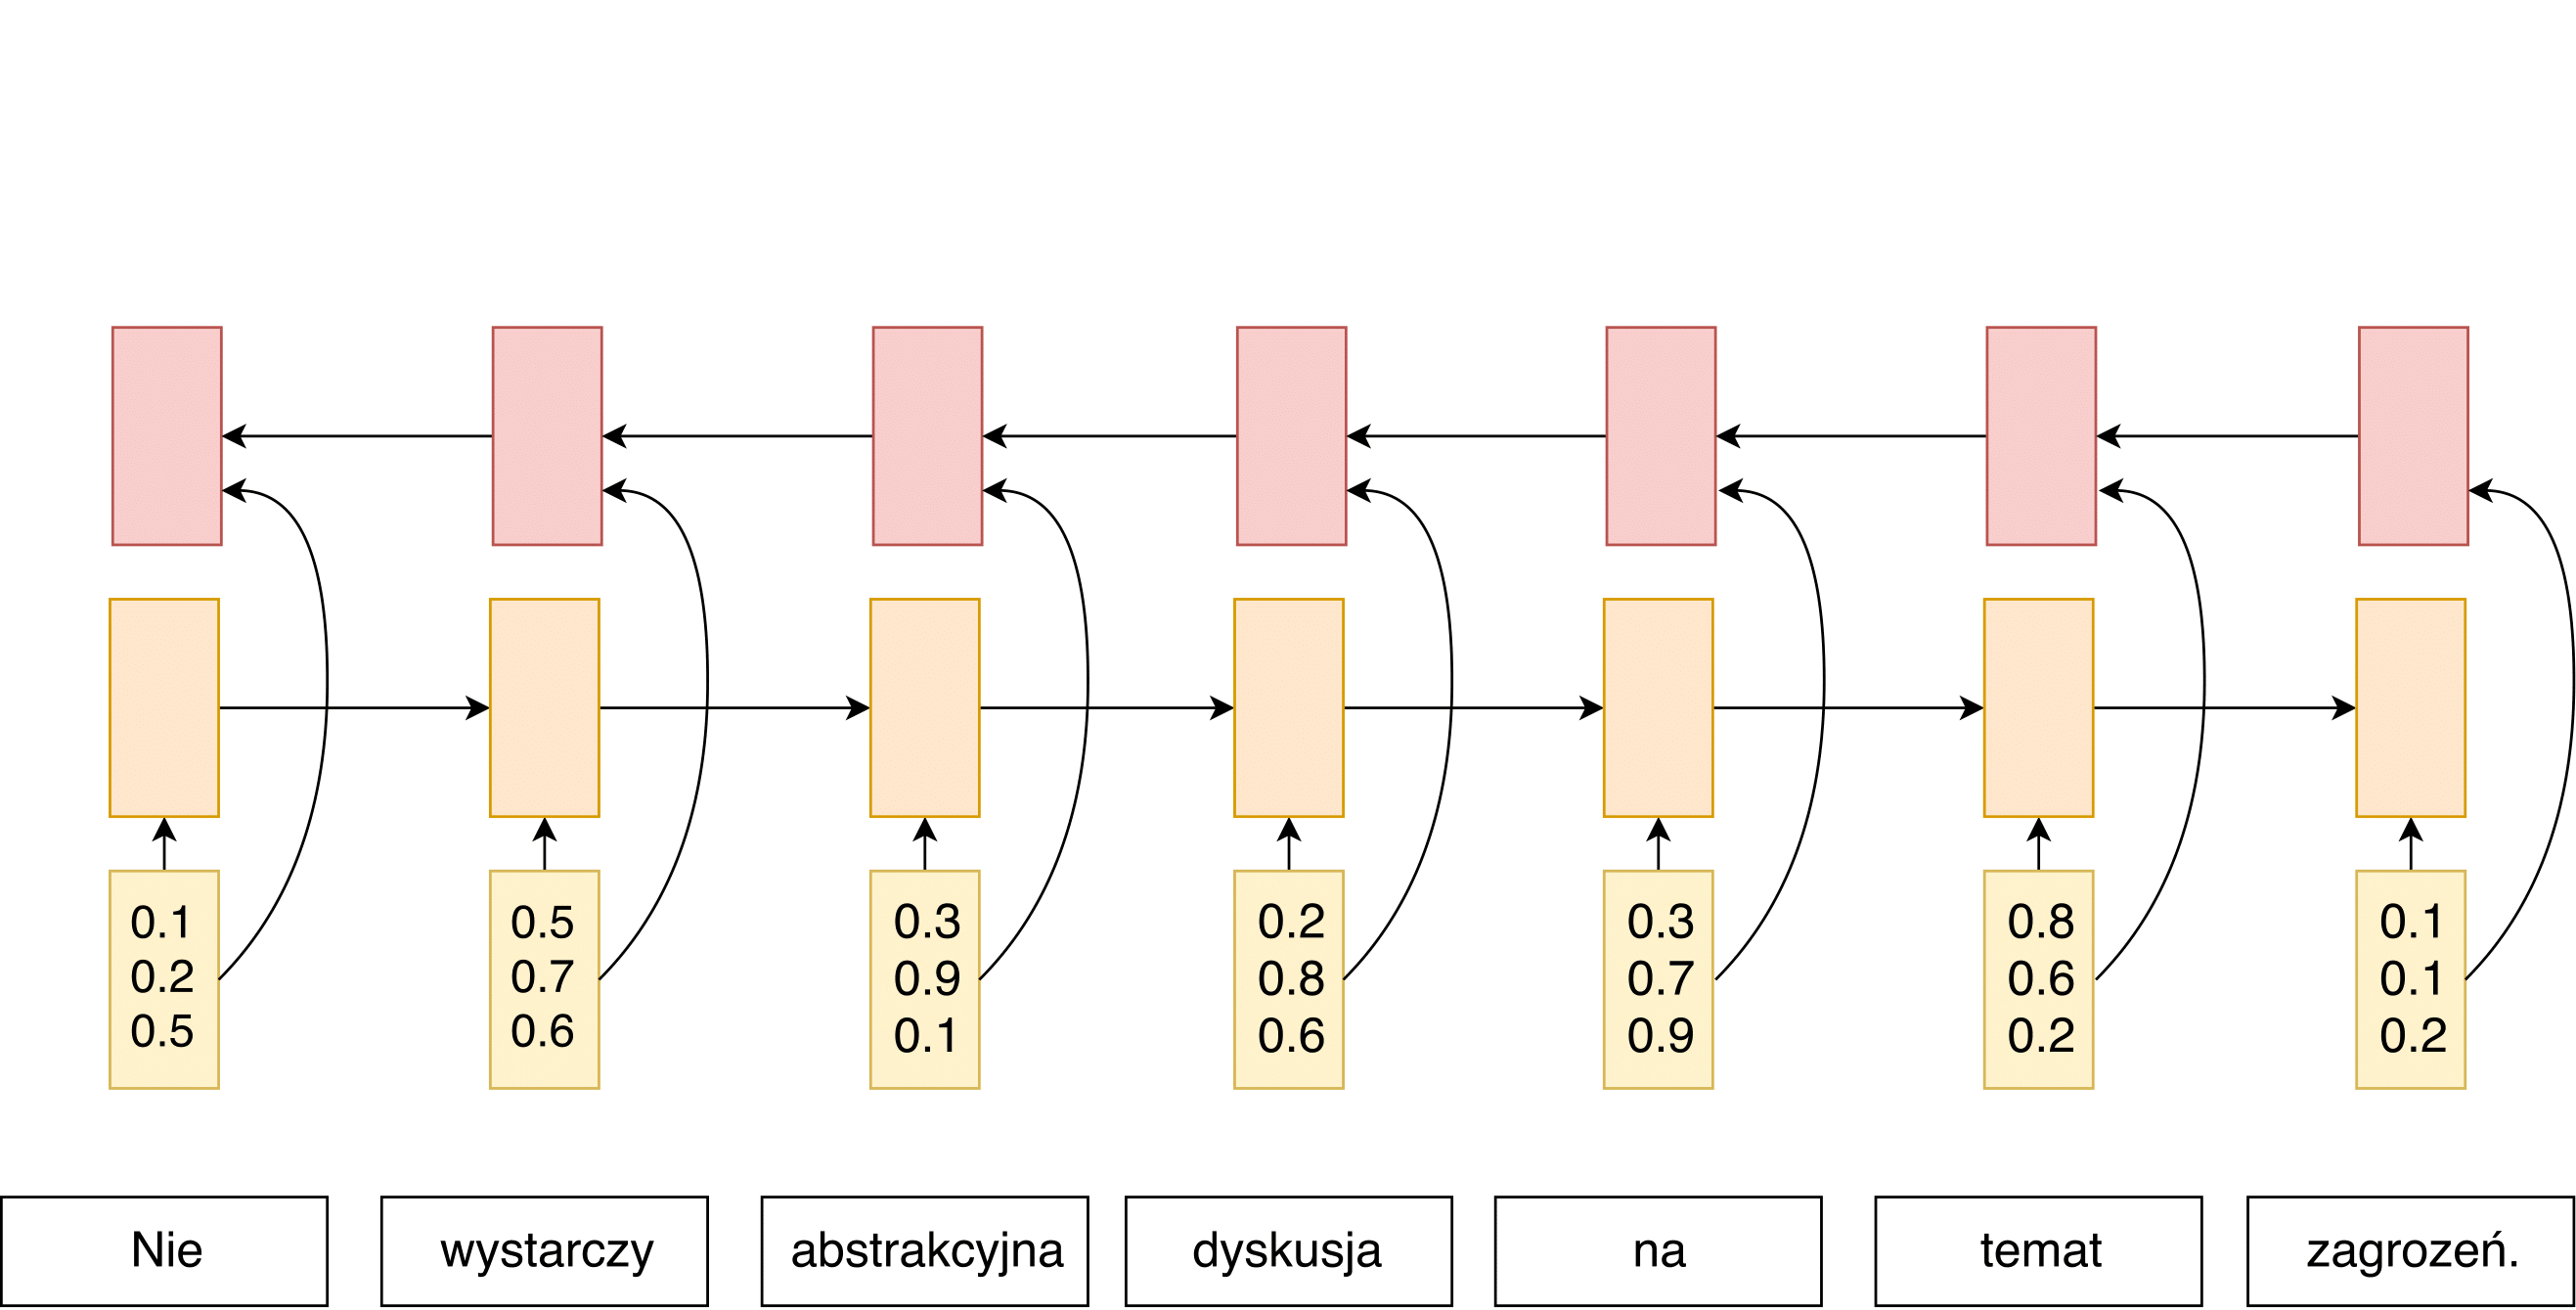
\includegraphics{./Encoder7-1.png}

    \hypertarget{lstm-long-short-term-memory}{%
\subsubsection{LSTM: Long Short Term
Memory}\label{lstm-long-short-term-memory}}

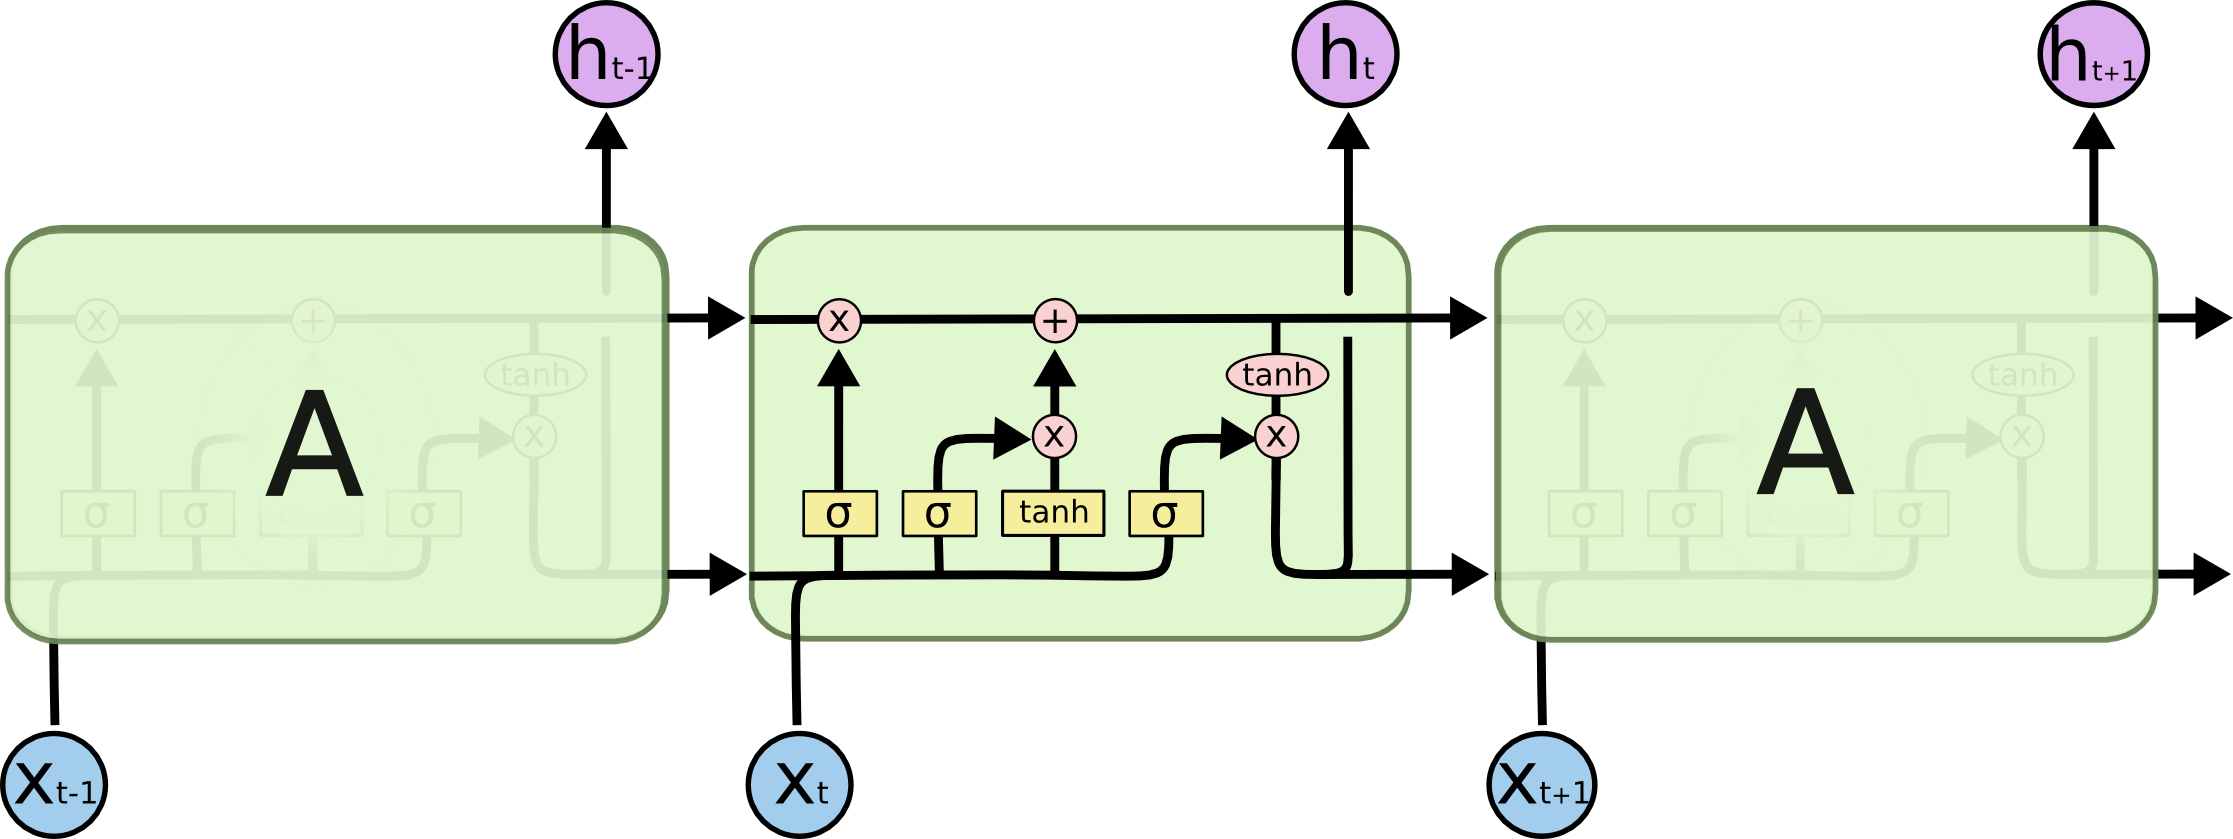
\includegraphics{./LSTM3-chain.png}

    \hypertarget{character-level-language-model}{%
\subsubsection{Character level Language
Model}\label{character-level-language-model}}

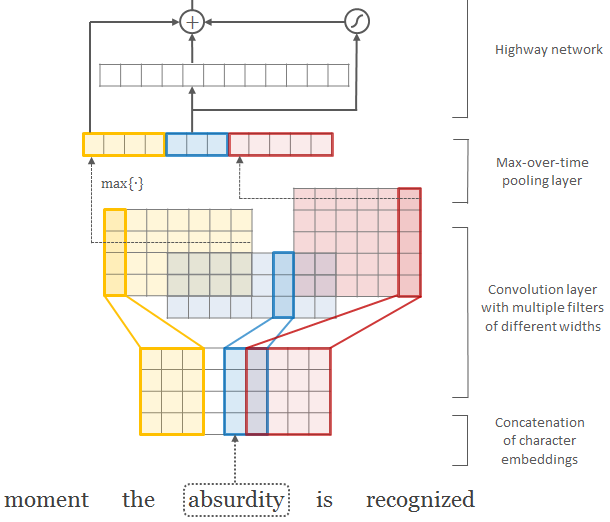
\includegraphics{./network.png}

    \hypertarget{fair-seq}{%
\subsubsection{FAIR seq}\label{fair-seq}}

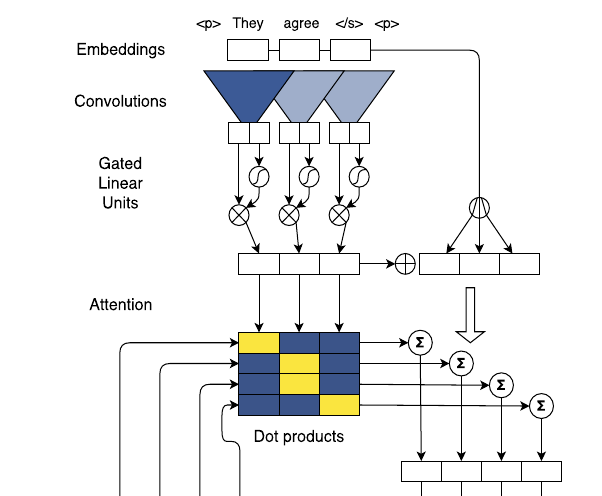
\includegraphics{./fair.png}

    \begin{Verbatim}[commandchars=\\\{\}]
{\color{incolor}In [{\color{incolor}60}]:} \PY{k+kn}{import} \PY{n+nn}{torch}
         \PY{k+kn}{import} \PY{n+nn}{torch}\PY{n+nn}{.}\PY{n+nn}{nn}\PY{n+nn}{.}\PY{n+nn}{functional} \PY{k}{as} \PY{n+nn}{F}
         \PY{k+kn}{from} \PY{n+nn}{sklearn}\PY{n+nn}{.}\PY{n+nn}{metrics} \PY{k}{import} \PY{n}{precision\PYZus{}recall\PYZus{}fscore\PYZus{}support}
         \PY{k+kn}{from} \PY{n+nn}{torch} \PY{k}{import} \PY{n}{nn}\PY{p}{,} \PY{n}{optim}
         \PY{k+kn}{from} \PY{n+nn}{torch}\PY{n+nn}{.}\PY{n+nn}{autograd} \PY{k}{import} \PY{n}{Variable}
         \PY{k+kn}{from} \PY{n+nn}{torch}\PY{n+nn}{.}\PY{n+nn}{nn}\PY{n+nn}{.}\PY{n+nn}{utils} \PY{k}{import} \PY{n}{weight\PYZus{}norm}
         \PY{k+kn}{from} \PY{n+nn}{torch}\PY{n+nn}{.}\PY{n+nn}{utils}\PY{n+nn}{.}\PY{n+nn}{data} \PY{k}{import} \PY{n}{DataLoader}\PY{p}{,} \PY{n}{TensorDataset}
\end{Verbatim}


    \hypertarget{bibliography-and-sources}{%
\subsubsection{Bibliography and
sources}\label{bibliography-and-sources}}

\begin{itemize}
\tightlist
\item
  \href{https://cs231n.github.io/convolutional-networks/}{Course on
  Stanford}
\item
  \href{https://adeshpande3.github.io/A-Beginner\%27s-Guide-To-Understanding-Convolutional-Neural-Networks/}{adeshpande3.github.io}
\item
  \href{http://ufldl.stanford.edu/tutorial/supervised/LogisticRegression/}{UFLDL}
\item
  \href{http://www.deeplearningbook.org/contents/convnets.html}{Chapter
  on CNN in Deep Learning book}
\item
  \href{https://papers.nips.cc/paper/4824-imagenet-classification-with-deep-convolutional-neural-networks.pdf}{AlexNet
  Paper}
\end{itemize}

    \hypertarget{thats-all-for-today}{%
\subsubsection{That's all for today!}\label{thats-all-for-today}}

\hypertarget{questions}{%
\subsubsection{Questions?}\label{questions}}


    % Add a bibliography block to the postdoc
    
    
    
    \end{document}
